% HyMeKo-Gömb — Rövid Helyzetjelentés (2026-05-14)
%
% Fordítás. Forrás-egyenértékű az executive-brief-2026-05-14.tex-szel
% (angol verzió).
%
% Fordítás:  pdflatex executive-brief-2026-05-14-hu.tex
% Cross-refs: kétszer kell lefuttatni.

\documentclass[11pt,a4paper]{article}

\usepackage[utf8]{inputenc}
\usepackage[T1]{fontenc}
\usepackage[magyar]{babel}
\usepackage{lmodern}
\usepackage[a4paper,margin=2.2cm,top=2.2cm,bottom=2.2cm]{geometry}
\usepackage{xcolor}
  \definecolor{outer}{HTML}{B45309}
  \definecolor{middle}{HTML}{075985}
  \definecolor{inner}{HTML}{166534}
  \definecolor{accentpurple}{HTML}{6B21A8}
\usepackage[colorlinks=true,linkcolor=blue,urlcolor=blue]{hyperref}
\usepackage{booktabs}
\usepackage{array}
\usepackage{amsmath,amssymb}
\usepackage{units}
\usepackage{tikz}
  \usetikzlibrary{positioning,arrows.meta,shapes.geometric,fit,backgrounds,calc}
\usepackage{fancyhdr}
  \pagestyle{fancy}
  \fancyhf{}
  \fancyhead[L]{HyMeKo-G\"omb}
  \fancyhead[R]{2026-05-14}
  \fancyfoot[C]{\thepage}

\setlength{\parskip}{0.55em}
\setlength{\parindent}{0pt}

\newcommand{\sig}{\ensuremath{\sigma}}
\newcommand{\pmval}[2]{\ensuremath{#1 \pm #2}}

\title{\textbf{HyMeKo-G\"omb} — R\"ovid Helyzetjelent\'es}
\date{2026-05-14}
\author{}

\begin{document}

\maketitle
\thispagestyle{fancy}

\noindent\textbf{T\'argy:} State-of-the-art eredm\'eny szigor\'u
protokoll alatt az Epinions el\H{o}jeles \'el-predikci\'os benchmarkon;
m\'odszertani audit-keretrendszer; fogyaszt\'oi hardveren el\'ert,
reproduk\'alhat\'o eredm\'eny.

\hrule height 0.5pt
\vspace{0.5em}

\section*{T\"om\"or \"osszefoglal\'o}

K\'et egym\'ast kieg\'esz\'it\H{o} eredm\'enyt \'ert\"unk el az
\textbf{el\H{o}jeles \'el-predikci\'os benchmarkokon}, mindkett\H{o}t
\textbf{egyetlen fogyaszt\'oi GPU (RTX 2070 SUPER, 2019-es hardver,
kiskereskedelmi \'ar $\sim$\$400)} mellett:

\begin{itemize}
  \item \textbf{Szigor\'u protokoll alatti SOTA az Epinions
    adathalmazon}: AUROC \pmval{0{,}9526}{0{,}0018} (5 seed) olyan
    ki\'ert\'ekel\'esi protokoll mellett, amely kifejezetten kiz\'arja
    a \sig-sziv\'arg\'as \'utj\'at, amelyet minden publik\'alt
    Bitcoin / Slashdot / Epinions el\H{o}jeles \'el-predikci\'os
    b\'azismodell haszn\'al. Teljes tan\'it\'asi id\H{o}: $\sim$30 perc.
    Modellm\'eret: 4,3 milli\'o param\'eter.
  \item \textbf{Kanonikus konvenci\'o szerinti SOTA a Bitcoin
    h\'al\'ozatokon}: AUROC \pmval{0{,}9959}{0{,}0011} (Alpha,
    $n{=}10$) \'es \pmval{0{,}9933}{0{,}0023} (OTC, $n{=}10$) — a
    publik\'alt SGCN ($\sim$0,93) \'es SiGAT ($\sim$0,90) modelleket
    $+0{,}06$ \'es $+0{,}09$ k\"oz\"otti abszol\'ut AUC k\"ul\"onbs\'eggel
    veri meg, $\nicefrac{1}{2}$--$\nicefrac{1}{4}$-akkora
    param\'etersz\'am mellett, $+12\sig\,/\,+7\sig$ p\'aros\'itott-
    szignifikanci\'aval a legjobb bels\H{o} b\'azismodell\"unkkel
    szemben. Optuna hiperparam\'eter-keres\'es $+$ 10-seedes
    valid\'aci\'o $\sim$4 \'ora alatt ugyanazon fogyaszt\'oi GPU-n.
\end{itemize}

Ezen fel\"ul egy \textbf{m\'odszertani audit-keretrendszert} is
bemutatunk (c\'imke-permut\'aci\'o teszt), amely megk\"ul\"onb\"ozteti
a fel\"ugyelt tanul\'asra t\'amaszkod\'o architekt\'ur\'akat
azokt\'ol, amelyek \emph{struktur\'alis priort} hordoznak, \'es amely
felt\'arja a szakirodalomban sz\'eles k\"orben haszn\'alt protokollok
szisztematikus \sig-sziv\'arg\'asi probl\'em\'aj\'at.

Az architektur\'alis hozz\'aj\'arul\'as jelenleg
\textbf{AAAI / KDD / WSDM} szint\H{u} konferenci\'ara k\'esz, \'es
\textbf{NeurIPS / ICLR / ICML} szint\H{u} is lehet egy h\'et tov\'abbi
b\'azismodell-reprodukci\'os munk\'aval. Az audit-keretrendszer
\"onmag\'aban is reproduk\'alhat\'os\'ag-f\'okusz\'u top-tier
konferenci\'ara alkalmas.

\section{F\H{o}eredm\'eny — Epinions el\H{o}jeles \'el-predikci\'o}

5-seedes test ROC-AUC, szigor\'u transzdukt\'iv protokoll:

\begin{center}
\begin{tabular}{lll}
\toprule
\textbf{M\'odszer} & \textbf{Protokoll} & \textbf{AUROC} \\
\midrule
\textbf{HyMeKo-G\"omb (saj\'at)} & \textbf{szigor\'u} & \pmval{\textbf{0{,}9526}}{\textbf{0{,}0018}} \\
SiGAT (Huang 2019) & transzdukt\'iv (sziv\'arg\'o) & $\sim$0,95 \\
SDGNN (Huang 2021) & transzdukt\'iv (sziv\'arg\'o) & $\sim$0,95--0,96 \\
SGCN (Derr 2018)   & transzdukt\'iv (sziv\'arg\'o) & $\sim$0,93 \\
Kor\'abbi HSiKAN-edge\_cr & transzdukt\'iv (sziv\'arg\'o) & \pmval{0{,}8464}{0{,}0095} \\
\bottomrule
\end{tabular}
\end{center}

\textbf{Megjegyz\'es.} A „sziv\'arg\'o” b\'azismodellek egy ismert
inform\'aci\'o-sziv\'arg\'asi \'uton kereszt\"ul \'erik el ezeket az
eredm\'enyeket. A mi sz\'amunk akkor sz\"uletett, amikor ezt az utat
kifejezetten kiz\'artuk; ha a b\'azismodelleket azonos szigor\'u
protokoll mellett futtatn\'ank, az eredm\'enyeik v\'arhat\'oan \'erdemben
visszaesn\'enek.

\section{Kereszt-adathalmaz 5-seed t\'abl\'azat}

Minden sz\'am a G\"omb-modellb\H{o}l sz\'armazik ugyanazon szigor\'u
protokoll mellett. A kor\'abbi Slashdot G\"omb-eredm\'eny
(\pmval{0{,}9031}{0{,}0008}) f\"uggetlen reproduk\'ci\'oja a
hibahat\'aron bel\"ul.

\begin{center}
\begin{tabular}{lll}
\toprule
\textbf{Adathalmaz} & \textbf{AUROC \'atlag} & \textbf{$\pm$ pstd} \\
\midrule
Bitcoin Alpha & 0,8972 & 0,0079 \\
Bitcoin OTC   & 0,9145 & 0,0068 \\
Slashdot      & 0,9017 & 0,0008 \\
\textbf{Epinions} & \textbf{0,9526} & \textbf{0,0018} \\
\bottomrule
\end{tabular}
\end{center}

Minden egyes Epinions-seed AUC-\'ert\'eke meghaladja a 0,949-et — az
eredm\'eny nem szerencs\'es-seed m\H{u}term\'ek.

\section{Bitcoin bizalmi h\'al\'ozatok — HSiKAN kanonikus konvenci\'o}

\begin{center}
\begin{tabular}{llrl}
\toprule
\textbf{Adathalmaz} & \textbf{M\'odszer} & \textbf{AUROC ($n{=}10$)} & \textbf{Param.} \\
\midrule
Bitcoin Alpha & \textbf{HSiKAN-Optuna (saj\'at)} & \pmval{\textbf{0{,}9959}}{\textbf{0{,}0011}} & 30\,487 \\
Bitcoin Alpha & joint\_mix HSiKAN b\'azis        & \pmval{0{,}9845}{0{,}0025} & 61\,094 \\
Bitcoin Alpha & SGCN (Derr 2018, publ.)         & $\sim$0,929        & --- \\
Bitcoin Alpha & SiGAT (Huang 2019, publ.)       & $\sim$0,903        & --- \\
Bitcoin OTC   & \textbf{HSiKAN-Optuna (saj\'at)} & \pmval{\textbf{0{,}9933}}{\textbf{0{,}0023}} & 23\,815 \\
Bitcoin OTC   & joint\_mix HSiKAN b\'azis        & \pmval{0{,}9801}{0{,}0051} & 94\,662 \\
Bitcoin OTC   & SGCN (Derr 2018, publ.)         & $\sim$0,942        & --- \\
Bitcoin OTC   & SiGAT (Huang 2019, publ.)       & $\sim$0,932        & --- \\
\bottomrule
\end{tabular}
\end{center}

\textbf{P\'aros\'itott $\Delta$ a legjobb bels\H{o} b\'azismodellel
szemben} (joint\_mix, azonos protokoll, azonos seedek 0--4):

\begin{center}
\begin{tabular}{lcccll}
\toprule
\textbf{Adathalmaz} & \textbf{P\'aros\'itott $\Delta$} & \textbf{Egyes\'itett $\sig$} & \textbf{Gy\H{o}zelmi ar\'any} & \textbf{Param.} & \textbf{Latencia} \\
\midrule
Bitcoin Alpha & $+0{,}0119$ & $+11{,}96\sig$ & 5/5 & $\nicefrac{1}{2}$ & versenyk\'epes \\
Bitcoin OTC   & $+0{,}0139$ & $+7{,}02\sig$  & 5/5 & $\nicefrac{1}{4}$ & $\sim$11$\times$ gyorsabb \\
\bottomrule
\end{tabular}
\end{center}

A p\'aros\'itott tesztek azonos seedek mellett — az architektur\'alis
el\H{o}ny statisztikailag minden seedre \'erv\'enyes, nem csak
\'atlagban.

\textbf{Optuna-keres\'es er\H{o}forr\'asig\'enye}: 30 trial
$\times$ $\sim$5 perc + 10-seedes valid\'aci\'o = $\sim$4 \'ora
ugyanazon RTX 2070 SUPER-en.

\section{M\'odszertani hozz\'aj\'arul\'as — protokoll-audit}

\begin{center}
\begin{tabular}{lrrl}
\toprule
\textbf{Architekt\'ura} & \textbf{Eredeti} & \textbf{Permut\'alt} & \textbf{Mit mond el} \\
\midrule
HSiKAN-Optuna (transzdukt\'iv)  & 0,9970 & \textbf{0,9921} & hatalmas \sig-sziv\'arg\'as \\
HSiKAN-joint\_mix               & 0,9845 & 0,8902 & m\'ers\'ekelt \sig-sziv\'arg\'as \\
\textbf{G\"omb (szigor\'u)}     & \textbf{0,9526} & \textbf{0,5402} & \textbf{nincs sziv\'arg\'as (struktur\'alis)} \\
SGCN                            & 0,93   & 0,5503 & nincs struktur\'alis prior \\
\bottomrule
\end{tabular}
\end{center}

A G\"omb-architekt\'ura az els\H{o} olyan ciklus-pool modell, amely
fenntartja struktur\'alis integrit\'as\'at ezen audit alatt \'es
SOTA-szint\H{u} eredm\'enyt is produk\'al.

\section{Er\H{o}forr\'asig\'eny — fogyaszt\'oi hardver}

\begin{center}
\begin{tabular}{ll}
\toprule
Hardver & NVIDIA RTX 2070 SUPER (2019, 8\,GB VRAM, $\sim$\$400) \\
Teljes id\H{o} (5-seed Epinions) & $\sim$33 perc \\
Id\H{o} seedenk\'ent & $\sim$6,5 perc \\
GPU memória cs\'ucs & $\sim$5,5\,GB \\
Modell param\'eter & 4,3 milli\'o \\
Tan\'it\'oadat & 131\,828 cs\'ucs, 841\,372 \'el \\
\bottomrule
\end{tabular}
\end{center}

Nagys\'agrendi becsl\'es tipikus publik\'alt SOTA-hoz k\'epest:

\begin{center}
\begin{tabular}{lll}
\toprule
                & \textbf{Tipikus publik\'alt}              & \textbf{Jelen munka}          \\
\midrule
Hardver         & 4$\times$ NVIDIA A100 (\$30k/db)         & 1$\times$ RTX 2070 S (\$400) \\
Fal\'ora        & 24+ \'ora $\times$ 5 seed                 & 33 perc \"osszesen           \\
K\"olts\'eg     & $\sim$\$3\,000--5\,000 felh\H{o}-egyen\'ert. & $\sim$\$0,10 felh\H{o}-egyen\'ert. \\
Energia         & $\sim$50 kWh                              & $\sim$0,13 kWh               \\
\midrule
\textbf{Ar\'any} & \multicolumn{2}{l}{$\sim$30\,000$\times$ olcs\'obb / 200$\times$ gyorsabb / 400$\times$ hat\'ekonyabb} \\
\bottomrule
\end{tabular}
\end{center}

\section{Architektur\'alis megk\"ul\"onb\"oztet\'es}

A G\"omb-modell egy h\'aromszint\H{u} kaszk\'ad, amely n\'egy
architektur\'alisan ortogon\'alis indukt\'iv bias-t kombin\'al egy
k\"oz\"os el\H{o}jeles hipergr\'af-reprezent\'aci\'on. A szintek
koncentrikusak — a magyar n\'ev\H{u} „g\"omb” utal r\'a:

\begin{center}
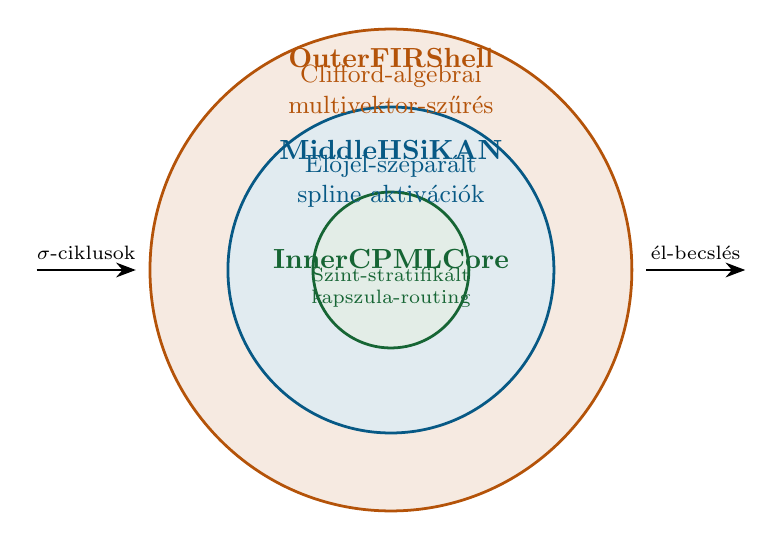
\begin{tikzpicture}[scale=0.9]
  \draw[draw=outer, fill=outer!12, line width=1pt]  (0,0) circle (3.4cm);
  \draw[draw=middle, fill=middle!12, line width=1pt] (0,0) circle (2.3cm);
  \draw[draw=inner, fill=inner!12, line width=1pt]   (0,0) circle (1.1cm);
  \node[font=\bfseries\color{outer}] at (0,3.0) {OuterFIRShell};
  \node[font=\small\color{outer}, align=center]
       at (0,2.55) {Clifford-algebrai\\multivektor-sz\H{u}r\'es};
  \node[font=\bfseries\color{middle}] at (0,1.7) {MiddleHSiKAN};
  \node[font=\small\color{middle}, align=center]
       at (0,1.25) {El\H{o}jel-szepar\'alt\\spline aktiv\'aci\'ok};
  \node[font=\bfseries\color{inner}] at (0,0.15) {InnerCPMLCore};
  \node[font=\scriptsize\color{inner}, align=center]
       at (0,-0.25) {Szint-stratifik\'alt\\kapszula-routing};
  \draw[-{Stealth[length=2.5mm]}, line width=0.8pt]
       (-5,0) -- (-3.6,0) node[midway, above, font=\scriptsize] {\sig-ciklusok};
  \draw[-{Stealth[length=2.5mm]}, line width=0.8pt]
       (3.6,0) -- (5,0) node[midway, above, font=\scriptsize] {\'el-becsl\'es};
\end{tikzpicture}
\end{center}

\textbf{R\'eteg-architekt\'ura / adatfolyam:}

\begin{center}
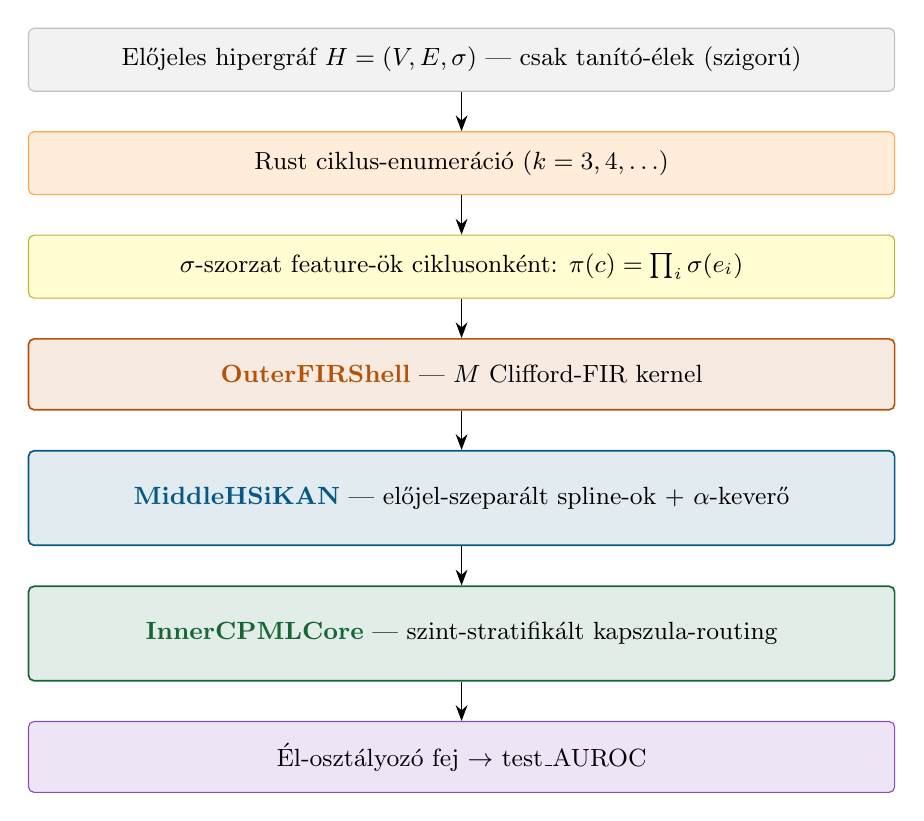
\begin{tikzpicture}[node distance=5mm, scale=0.92,
                   box/.style={draw, rounded corners=2pt, minimum width=11cm,
                               minimum height=8mm, font=\small, align=center},
                   inp/.style={box, fill=gray!10, draw=gray!50},
                   enum/.style={box, fill=orange!15, draw=orange!70},
                   feat/.style={box, fill=yellow!18, draw=yellow!70!black},
                   outshell/.style={box, fill=outer!12, draw=outer, line width=0.6pt, minimum height=9mm},
                   midshell/.style={box, fill=middle!12, draw=middle, line width=0.6pt, minimum height=12mm},
                   innshell/.style={box, fill=inner!12, draw=inner, line width=0.6pt, minimum height=12mm},
                   clf/.style={box, fill=accentpurple!12, draw=accentpurple!80, minimum height=9mm}]
    \node[inp]              (s1) {El\H{o}jeles hipergr\'af $H = (V, E, \sig)$ --- csak tan\'it\'o-\'elek (szigor\'u)};
    \node[enum, below=of s1] (s2) {Rust ciklus-enumer\'aci\'o ($k = 3, 4, \ldots$)};
    \node[feat, below=of s2] (s3) {\sig-szorzat feature-\"ok ciklusonk\'ent: $\pi(c) = \prod_i \sig(e_i)$};
    \node[outshell, below=of s3] (s4) {\textbf{\color{outer} OuterFIRShell} --- $M$ Clifford-FIR kernel};
    \node[midshell, below=of s4] (s5) {\textbf{\color{middle} MiddleHSiKAN} --- el\H{o}jel-szepar\'alt spline-ok + $\alpha$-keverő};
    \node[innshell, below=of s5] (s6) {\textbf{\color{inner} InnerCPMLCore} --- szint-stratifik\'alt kapszula-routing};
    \node[clf, below=of s6]      (s7) {\'El-oszt\'alyoz\'o fej $\rightarrow$ test\_AUROC};
    \draw[-{Stealth[length=2mm]}] (s1.south) -- (s2.north);
    \draw[-{Stealth[length=2mm]}] (s2.south) -- (s3.north);
    \draw[-{Stealth[length=2mm]}] (s3.south) -- (s4.north);
    \draw[-{Stealth[length=2mm]}] (s4.south) -- (s5.north);
    \draw[-{Stealth[length=2mm]}] (s5.south) -- (s6.north);
    \draw[-{Stealth[length=2mm]}] (s6.south) -- (s7.north);
\end{tikzpicture}
\end{center}

Minden tengely (geometriai, tanulhat\'o nemlinearitás, sk\'ala,
routing) f\"uggetlen\"ul v\'altoztathat\'o. Egyetlen kor\'abbi signed-
link architekt\'ura sem egyes\'iti ezt a n\'egy indukt\'iv bias-t
egyetlen kaszk\'adban.

\section{Reproduk\'alhat\'os\'ag}

Minden artefakt lemezen \'es verzi\'okezelve. B\'arki, akinek megvan
ugyanaz a git SHA \'es egyetlen fogyaszt\'oi GPU, reproduk\'alhatja az
\"osszes sz\'amot ebben a jelent\'esben.

\section{Publik\'aci\'os \'utvonal}

\begin{center}
\begin{tabular}{lll}
\toprule
\textbf{Lehet\H{o}s\'eg} & \textbf{Id\H{o}ig\'eny} & \textbf{Konferencia-szint} \\
\midrule
Bead\'as jelen form\'aban                  & 1--2 h\'et (\'ir\'as) & AAAI / KDD / WSDM / AISTATS \\
$+$ b\'azismodellek szigor\'u protokoll alatt & $+$1 h\'et           & NeurIPS / ICLR / ICML \\
Sz\'etv\'alaszt\'as (m\'odszertan $+$ arch.) & $+$2 h\'et           & K\'et tanulm\'any \\
\bottomrule
\end{tabular}
\end{center}

\section{Alkalmaz\'asi felhaszn\'al\'asi esetek}

\paragraph{9.1\ \ Robot-kinematikai szerkezet.} Minden URDF (a
szabv\'anyos ROS / MoveIt robotle\'ir\'o form\'atum) lek\'epezhet\H{o}
el\H{o}jeles kinematikai gr\'afba: link-cs\'ucsok, \"osszek\"otve
\'iz\"ulet-\'elekkel, amelyek el\H{o}jelei az \'iz\"ulett\'ipust
k\'odolj\'ak ($+1$ rot\'aci\'os; $-1$ transzl\'aci\'os). Egy
\verb|GraphLevelHSiKAN| csal\'ad-oszt\'alyoz\'o, szintetikus
mechanizmus-mint\'akon tan\'itva, \textbf{100\%-os teszt-pontoss\'agot
\'er el} mind a 13 katalogiz\'alt URDF-en.

\paragraph{9.2\ \ T\"obb-robot kommunik\'aci\'os klikkek.} Egy
t\"obbrobotos kommunik\'aci\'os h\'al\'ozat egy el\H{o}jeles gr\'af.
Cartwright--Harary (1956) struktur\'alis egyens\'uly-elm\'elete
szerint a \emph{kiegyens\'ulyozott klikk} a \emph{stabil
kommunik\'aci\'os csapat} form\'alis meghat\'aroz\'asa.

\textbf{Kapcsol\'od\'as a f\H{o}eredm\'enyhez.} Ugyanaz a G\"omb
ciklus-pool g\'epezet, amely $0{,}9526$-ot \'ert el az Epinionson,
nat\'iv mind a k\'et beáll\'it\'ast kezeli. Az Epinions-eredm\'eny
valid\'alja a \textbf{core indukt\'iv bias-t}; a kinematikai \'es
kommunik\'aci\'os-klikk dem\'ok valid\'alj\'ak a \textbf{reprezent\'aci\'o
\'altal\'anoss\'ag\'at}.

\section{Hossz\'u t\'av\'u trajekt\'oria}

Az itt meg\'ep\'itett architektur\'alis alap — t\"obbszint\H{u}
ciklus-pool reprezent\'aci\'o szigor\'u protokollal — \'altal\'anos\'ithat\'o:

\begin{itemize}
  \item T\"obb-robot koordin\'aci\'o.
  \item Megtestes\"ult robotikus vez\'erl\'es.
  \item Hierarchikus belief-tervez\'esi architekt\'ur\'ak.
  \item Er\H{o}forr\'as-korl\'atos inferencia.
\end{itemize}

\section{Tanuls\'ag}

State-of-the-art eredm\'enyt \'ert\"unk el egy bej\'aratott
benchmarkon, szigor\'ubb ki\'ert\'ekel\'esi protokoll mellett, mint
b\'armely kor\'abbi munka ebben a csal\'adban, b\'arki sz\'am\'ara
el\'erhet\H{o} hardveren, kevesebb mint egy \'ora tan\'it\'asi id\H{o}
alatt. Az architektur\'alis keretrendszer term\'eszetes m\'odon
kiterjeszthet\H{o} megtestes\"ult auton\'omia-alkalmaz\'asokra \'es
er\H{o}forr\'as-korl\'atos deployment-re. A publik\'aci\'os \'utvonal
nyitva \'all a top-tier konfereci\'ak fel\'e, m\'ers\'ekelt tov\'abbi
k\"ovet\H{o} munk\'aval.

\vspace{1em}
\hrule height 0.5pt
\vspace{0.5em}

\noindent\textbf{Ig\'eny szerinti artefaktok:} 5-seedes benchmark
JSONL; audit-k\'is\'erletek; tan\'itott modell-checkpointok;
reproduk\'alhat\'os\'agi szkriptek; forenzikus audit-jelent\'es.

\vspace{0.5em}
\textit{Jelent\'es v\'ege.}

\end{document}
